\chapter{Analyse af Lotka-Volterra's rovdyr-byttedyr model}
I dette afsnit søger vi at analysere systemet ved hjælp af nulkliner, ligevægtspunkter og fasediagrammer. Det skal være med til at skabe et indblik i, hvordan systemet opfører sig og skal ligge til grund for en udvidelse af modellen.\\
\section{Lotka-Volterra}
Vi har Lotka-Volterra's model med notation som nedenstående. Dette er et autonomt og ikke-lineært system, og dets eksakte løsning ligger uden for projektets rammer. Det ønskes derfor at se kvalitativt og analytisk på systemet:
\begin{equation}
    \begin{aligned}
    b'(t) = (A-Br(t)) b(t),\\
    r'(t) = (Db(t)-C) r(t)
    \end{aligned}
    \label{IVPlovo}
\end{equation}

med begyndelsesværdibetingelserne

\begin{equation}\label{LoVoIVP}
    \begin{cases}
    b(t_0)&= b_0 \ , \ b_0\geq0\\
    r(t_0)&= r_0 \ , \ r_0\geq0
    \end{cases}
\end{equation}

Her indføres de to hjælpefunktioner $j$ og $l$. 
\begin{align}
    j(b,r) &= Ab - Brb\label{bytteh}\\
    l(b,r) &= Dbr - Cr
    \label{rovh}
\end{align}

Vi vil nu vise, at Lotka-Volterra's model opfylder betingelserne i EESFS, da det fremadrettet kan benyttes som et argumentationsværktøj med hensyn til løsningskurverne.
\begin{lemma}{Anvendelse af EESFS på Lotka-Volterra's model}{}
EESFS kan anvendes på Lotka-Volterra's model som vist i systemet \eqref{IVPlovo} med begyndelsesværdibetingelserne \eqref{LoVoIVP}:
%\begin{equation*}
%    \dot{y}=\vec{f}(t,\vec{y})=
%    \begin{cases}
%    j(b,r)&=Ab-Brb\\
%    l(b,r)&=Dbr-Cr
%    \end{cases}
%    \ ,\ \textnormal{hvor} \ 
%    \begin{cases}
%    b(t_0)&= b_0\\
%    r(t_0)&= r_0
%    \end{cases}
%\end{equation*}
\end{lemma}

\begin{proof}\\
Vi tjekker, at de tre betingelser i EESFS er opfyldt.\\ \hfill \break
\begin{enumerate}
    \item Vektorfunktionen, $\vec{f}(\vec{b},\vec{r})=(j(b,r),l(b,r))$, er defineret og kontinuert på hele $\mathbb{R}^3$, da $t$ ikke indgår eksplicit, og både $j$ og $l$ er definerede på hele $\mathbb{R}^2$. Vi har altså, at $\vec{f}\colon \mathbb{R}\times \mathbb{R}^2\to\mathbb{R}^3$.
    \item De partielle afledede eksisterer og er givet ved:
    \begin{equation*}
    \frac{\partial\vec{f}}{\partial \vec{y}}=
    \begin{bmatrix}
    \frac{\partial j}{\partial b} & \frac{\partial j}{\partial r}\vspace{1mm}\\
    \frac{\partial l}{\partial b} & \frac{\partial l}{\partial r}
    \end{bmatrix}
    =
    \begin{bmatrix}
    A-Br & -Bb\\
    Dr & Db-C
    \end{bmatrix}
    \end{equation*}
    Det ses, at alle de partielle afledede er førstegradspolynomier, og dermed er $\frac{\partial\vec{f}}{\partial \vec{y}}$ kontinuert.
    \item Kravet til begyndelsesbetingelsen er trivielt opfyldt, da $\vec{f}$ er defineret på hele $\mathbb{R}^3$.
\end{enumerate}
\end{proof}

\hfill \break

For at finde nulklinerne for de to hjælpefunktioner $j$ og $l$, skal vi først omskrive vores funktioner, hvorefter nulreglen kan anvendes:

\begin{align*}
    j(b,r)&=Ab-Bbr  &   l(b,r)&=-Cr+Drb\\
    &=Bb\left(\frac{A}{B}-r\right)  &   &=Dr\left(b-\frac{C}{D}\right)
\end{align*}

Da er $j$-nulklinen givet ved den horisontale linje $r=\frac{A}{B}$ og $r$-aksen, og $l$-nulklinen er givet ved den vertikale linje $b=\frac{C}{D}$ og $b$-aksen. \\
\hfill \break
I det følgende vil vi vise at hvis $b_0>0$ og $r_0>0$, så vil løsningskurverne for systemet ligge i første kvadrant. \\
\hfill \break
Lad $b_1 \geq 0$ og $t_1\in \mathbb{R}$ være givet. Vi ønsker at konstruere en løsning, som går gennem punktet $(b_1,0)$ til tiden $t_1$. Hvis $r(t)\equiv 0$, så ses det, at $b(t)=b_1e^{A(t-t_1)}$ er en sådan løsning, som ligger på $b$-aksen for alle $t$. Grundet EESFS er der ikke andre løsninger, som går gennem punktet $(b_1,0)$ til tiden $t_1$. Da $b_1$ og $t_1$ var arbitrære, kan en sådan løsning konstrueres over hele $b$-aksen. En løsning, med begyndelsespunkt i 1. kvadrant, kan således ikke krydse den positive del af $b$-aksen. \\ 
\hfill \break
 Lad nu $r_1 \geq 0$ og $t_1 \in \mathbb{R}$ være givet. Hvis $b(t)\equiv 0$, så vil $r(t)=r_1e^{-C(t-t_1)}$ være en løsning, som ligger på $r$-aksen for alle $t$, som går gennem $(0,r_1)$ til tiden $t_1$. Af samme grund som før, kan en løsning med begyndelsespunkt i 1. kvadrant derfor ikke krydse den positive del af $r$-aksen, og dermed kan løsningskurven ikke forlade 1. kvadrant. 
\\ 
\hfill \break
Vi ønsker derfor kun at analysere på det indre af 1. kvadrant. Denne opdeles i 4 områder af $j$ og $l$ nulklinerne. Disse 4 områder vil i det følgende betegnes som; $O_1, O_2, O_3$ og $O_4$, hvor disse områder nummereres analogt med kvadranterne i et kartesisk koordinatsystem, hvor punktet $( \frac{C}{D},\frac{A}{B})$ betragtes som origo. Vi har altså:
\begin{align*}
    O_1 &= \left\{(b,r) \in \mathbb{R}^2 | b > \frac{C}{D}, r > \frac{A}{B}\right\}\\
    O_2 &= \left\{(b,r) \in \mathbb{R}^2 | b < \frac{C}{D}, r > \frac{A}{B}\right\}\\
    O_3 &= \left\{(b,r) \in \mathbb{R}^2 | b < \frac{C}{D}, r < \frac{A}{B}\right\}\\
    O_4 &= \left\{(b,r) \in \mathbb{R}^2 | b > \frac{C}{D}, r < \frac{A}{B}\right\}.
\end{align*}
\hfill \break
 Det er klart, at funktionerne $j(b,r), l(b,r)$ er monotone, endda strengt monotone i de 4 områder, og vi kan analysere, hvorvidt populationerne er voksende eller aftagende i hvert område. Lad os først betragte et punkt $(b_0,r_0)$ i $O_1$. Da gælder følgende:
\begin{align*}
    j(b_0, r_0) &= Bb_0\left(\frac{A}{B} - r_0 \right)\\
    j(b_0, r_0) &< 0
\end{align*}
og
\begin{align*}
    l(b_0, r_0) &= Dr_0\left(b_0 - \frac{C}{D} \right)\\
    l(b_0, r_0) &> 0
\end{align*}
En analog fremgangsmåde kan køres igennem for de andre regioner for at bestemme, hvorvidt $j(b,r)$ og $l(b,r)$ er voksende eller aftagende, og dette giver følgende fasediagram.\\
\hfill \break

\begin{figure} [H]
    \centering
    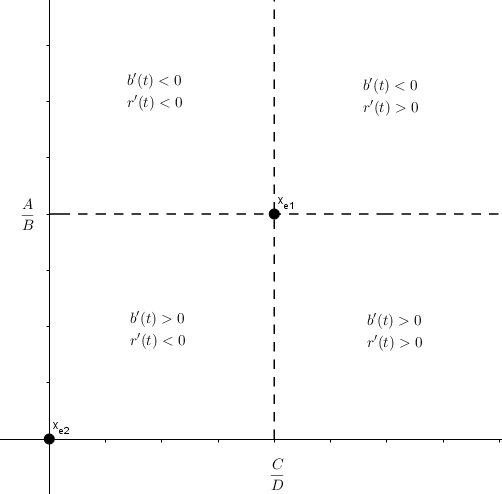
\includegraphics[scale=0.5]{Images/lvnull.png}
    \caption{Nullkliner \citep[s. 24]{Svensk}}
    \label{null}
\end{figure}

Af nulklinerne ses det, at punktet:
$$\left(\frac{C}{D}, \frac{A}{B}\right)=y^*_1$$
er et ligevægtspunkt, mens $(0,0)=y^*_2$ også er et ligevægtspunkt.\\ \hfill \break
Tangenthældningen i et punkt $(b(t_0), r(t_0))$ er, jævnfør ligning \eqref{dydt}, givet ved $\frac{r'(t_0)}{b'(t_0)}$.


Vi betragter tilfældet $r<\frac{A}{B}$. Så gælder det, at $r$ er en funktion af $b$, da $b(t)$ er bijektiv i dette område. Da ses det, at $b(t)$ har en invers, og $t$ kan derfor betragtes som en funktion af $b$, $t(b)$. Deraf fås, at $r'(b) = r'(t(b))$. Vi kan altså skrive tangenthældningen:
$$\textnormal{tangenthældningen}=\frac{\frac{dr}{dt}}{\frac{db}{dt}}=\frac{r(t)(-C+D\cdot b(t))}{b(t)(A-B\cdot r(t))}$$

hvor $\frac{db}{dt}\neq 0$, da $r<\frac{A}{B}$. Dette er en separabel differentialligning, og da $r,b > 0$ giver nedenstående ikke anledning til problemer.
\begin{equation}
    \frac{A-B\cdot r}{r}\cdot \frac{dr}{db}= \frac{-C+D\cdot b}{b}.
\label{r(t)ogb(t)}
\end{equation}

Løsningen til ligning \eqref{r(t)ogb(t)} er
\begin{equation}\label{mikkel}
   A\cdot \ln(r)-Br=-C\ln(b)+Db+K',
\end{equation}
hvilket også kan skrives
\begin{align}
r^Ae^{-Br}=Kb^{-C}e^{Db},
\label{solve}
\end{align}
hvor $K=e^{K'}$. Det samme er gældende for $r>\frac{A}{B}$. Vi ønsker nu at undersøge tilfældet $r=\frac{A}{B}$. I dette tilfælde er $\frac{db}{dt}=0$, og ovenstående fremgangsmåde kan ikke bruges. \\
 Vi kan for $b<\frac{C}{D}$ betragte $b$ som en funktion af $r$, med samme argument som før. Hvis vi bytter om på $b$-aksen, og $r$-aksen, følger det af ligning \eqref{dydt}, at tangenthældningen er givet ved: $$\frac{db}{dr}=\frac{b(A-B\cdot r)}{r(-c+D\cdot b)}$$
 Dette er den samme separable differentialligning som i ligning \eqref{r(t)ogb(t)}. Dermed er løsningen også givet ved ligning \eqref{solve}. Det samme er gældende for $b>\frac{C}{D}$. Vi mangler nu bare at betragte tilfældet, hvor $b=\frac{C}{D}$ og $r=\frac{A}{B}$. Men dette punkt er et ligevægtspunkt for systemet, så den eneste løsning i punktet er den konstante løsning.
 
 Der er altså i ligning \eqref{solve} givet en funktion $z(r)$ på venstresiden og en funktion $w(b)$ på højresiden:
\begin{equation} \label{zr}
    z(r)=r^Ae^{-Br}, r>0
\end{equation}

\begin{equation} \label{wb}
    w(b)=Kb^{-C}e^{Db}, b>0
\end{equation}
    


Disse to funktioner vil være lig med hinanden til ethvert punkt på faseportrættet i 1. kvadrant. Dermed kan fasediagrammet udvides således:\\
\begin{figure} [H]
    \centering
    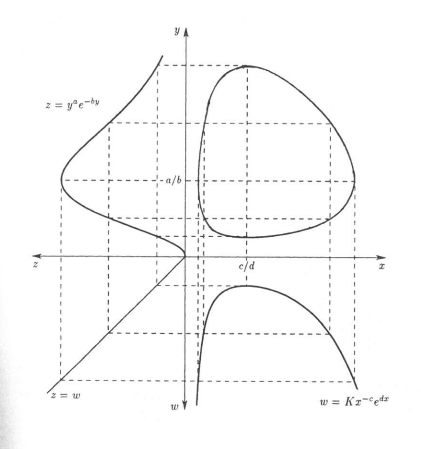
\includegraphics[scale=0.8]{Images/fasediagramteori.png}
    \caption{Her sættes $y=r$ og $x=b$. Figuren er taget fra \citep[s. 25]{Svensk}.}
    \label{svensk}
\end{figure}


%Da faseportrættet for (\ref{solve}) er enten en lukket kurve, et punkt eller en tom graf, for ethvert $K$, kan løsningerne til systemet bestående af (\ref{bytte}) og (\ref{rov}) beskrives som lukkede kurver i $br$-planet. \\

Figur \ref{svensk} undersøges nu ved hjælp af ligningerne; \eqref{solve}, \eqref{zr} og \eqref{wb}. Denne undersøgelse opdeles i fire, hvor der ses isoleret på hver kvadrant. I 1. kvadrant er fasediagrammet for modellen afbilledet, i 2. kvadrant ses grafen for \eqref{zr}, i 3. kvadrant er grafen for \eqref{solve} afbilledet, og 4. kvadrant viser grafen for \eqref{wb}:
\begin{enumerate}
    \item I dette punkt undersøges 4. kvadrant i figur \ref{svensk}. 
    
    Grænseværdien for ligningen, $w(b) = K b^{-C} e^{Db}$ for $b \in  \left] 0, \infty \right[$, undersøges. Her deles analysen af grænseværdier op i to tilfælde; tilfælde 1, hvor $b \to 0^+$, og tilfælde 2, hvor $b \to \infty$. I ligningen er $C, D \ \textnormal{og} \ K$ positive konstanter.\\
    \hfill \break
    $b \to 0^{+}$:  \\
    Her vil $e^{Db} \to 1$, og $b^{-C}\to \infty \ \textnormal{for} \ b \to 0^+$. Da K er en positiv konstant, vil den ikke ændre på grænseværdien for $w(b)$, og dermed gælder $w(b)=K b^{-C} e^{Db} \to \infty, \ \textnormal{for} \ b \to 0^+.$ \\
    
    $b \to \infty$:\\
    $w(b)$ omskrives til 
    \begin{equation}\label{flh1}
        K \left( \frac{e^{b \frac{D}{C}}}{b} \right)^C,
    \end{equation}
    hvorpå L' hôpitals regel om $\infty/\infty$-udtryk \citep[sætning 7.23 s. 125]{Analyse bog} anvendes på inderste udtryk:
    \begin{equation} \label{lh1}
        \frac{\frac{D}{C} e^{b\frac{D}{C}}}{1}.
    \end{equation}
    %Udfra ovenstående ses det nu, at forholdet mellem tæller og nævner i \eqref{lh1} går mod $\infty$, hvormed $e^{Db} \to \infty \ \textnormal{og} \ b^{- C} \to \infty \ \textnormal{for} \ b \to \infty$.
    Dette vil for $b \to \infty$, gå imod uendelig, og eftersom $K$ er en positiv konstant, vil den derfor ikke ændre på grænseværdien. Derfor gælder, at $K \left(\frac{\frac{D}{C} e^{b\frac{D}{C}}}{1}\right)^C\to \infty \ \textnormal{for} \ b \to \infty$.
    Ud fra L'hôpitals regel \citep[sætning 7.23 s. 125]{Analyse bog} vil $K \left( \frac{e^{b \frac{D}{C}}}{b} \right)^C \to \infty$ for $b \to \infty$. Hvormed $w(b) \to \infty \ \textnormal{for} \ b \to \infty$.\\
   
   Det vides udfra de to ovenstående tilfælde, at $w(b)$ er nedadtil begrænset, og Pér \citep[korollar 7.16, s. 121]{Analyse bog} vil der for ligningen eksistere et globalt ekstremum. Da funktionen $w(b) \to \infty \ \textnormal{for både} \ b\to 0^+$ og $b \to \infty$, vil der til et bestemt $b$ optræde et $\inf{w(b)}$. Dette infimum for $w(b)$ optræder, når $w'(b) = 0$. $w'(b)$ bestemmes:

$$w'(b)=\frac{-Kb^{-C}C\mathrm{e}^{Db}}{b}+Kb^{-C}D\mathrm{e}^{Db}.$$

Denne sættes lig nul, og der isoleres for b: 

\begin{equation}
    b=\frac{C}{D}.
\end{equation}

Der kan altså konkluderes, at $w(b) \to \infty$, for henholdsvis $b \to 0^+$ og $b \to \infty$. Derudover er det globale minimum for funktionen bestemt til at være $\inf{w(b)}= w \left(\frac{C}{D} \right)$. Dermed er grafen for 4. kvadrant i figur \ref{svensk} beskrevet. \\
    
    \item  I dette punkt undersøges 2. kvadrant i figur \ref{svensk}.
    
    Grænseværdien for ligningen, $z(r) = r^A e^{-Br}$ for $r \in \left]0,\infty \right[$, undersøges.
 Her deles analysen af grænseværdier op i to tilfælde; tilfælde 1, hvor $r \to 0^+$, og tilfælde 2, hvor $r \to \infty$. I ligningen er $A \ \textnormal{og} \ B$ positive konstanter.\\
 \hfill \break

    $r \to 0^+$:\\
    Da vil $r^A \to 0$, og $e^{-Br} \to 1$ for $r \to 0^+ $. Dermed gælder, at $z(r)=r^A e^{-Br} \to 0 \ \textnormal{for} \ r \to 0^+$ \\

    $r \to \infty$: \\
   $z(r)$ omskrives til
   \begin{equation*}
       \left(\frac{r}{e^{\frac{B}{A}r}} \right)^A
   \end{equation*}
   og herpå anvendes L' hôpitals regel om $\infty/\infty$-udtryk \citep[sætning 7.23 s. 125]{Analyse bog} på inderste udtryk:
    $$\frac{1}{\frac{B}{A}e^{\frac{B}{A}r}}.$$
    
    Da $\frac{B}{A}e^{\frac{B}{A}r} \to \infty$ for $r \to \infty$, og $1$ er konstant, vil $\frac{1}{\frac{B}{A}e^{\frac{B}{A}r}} \to 0$ for $r \to \infty.$
    Ud fra L'hôpitals regel \citep[sætning 7.23 s. 125]{Analyse bog} vil $z(r) \to 0$ for $r \to \infty$. 

Det vides ud fra de to ovenstående tilfælde, at $z(r)$ er opadtil begrænset, og Pér \citep[korollar 7.16, s. 121]{Analyse bog} vil der for ligningen eksistere et globalt ekstremum. Da funktionen $z(r) \to 0 \ \textnormal{for både} \ r \to 0^+$ og $r \to \infty$, vil der til et bestemt $r$ optræde et $\sup{z(r)}$. Dette supremum for ligning \eqref{zr} optræder, når $z'(r) = 0$. $z'(r)$ bestemmes:
$$z'(r)=\frac{Ar^A\mathrm{e}^{-Br}}{r}-r^AB\mathrm{e}^{-Br}$$

Denne sættes lig nul, og der isoleres for r:
$$r = \frac{A}{B}.$$

Der kan altså konkluderes, at $z(r) \to 0$, for henholdsvis $r \to 0^+$ og $r \to \infty$. Derudover er maksimum for funktionen bestemt til at være $\sup{z(r)}= z \left(\frac{A}{B} \right)$. Dermed er grafen for 2. kvadrant i figur \ref{svensk} beskrevet. \\

\item I det følgende vil vi beskrive 3. kvadrant i figur \ref{svensk}, hvor $w(b) = z(r)$, og hældningskoefficienten er dermed $1$. Denne beskriver altså forholdet mellem $w(b)$ og $z(r)$. Det vides udfra undersøgelsen af $w(b)$ at, denne antager $\inf{w(b)}$ ved $b=\frac{C}{D}$, her vil $z(r)$ således også antage minimum, når $z(r_{min}) = z(r_{max})$. Det samme gør sig gældene for $\sup{z(r)}$ når $r= \frac{A}{B}$, hvorved $w(b)$ ligeledes antager maksimum, ved $w(b_{min}) = w(b_{max})$. Det er med andre ord denne sammenhæng, der gør det muligt at konstruere de stiplede linjer i figur \ref{svensk}.

\item Her vil fasediagrammet i 1. kvadrant undersøges ved brug af undersøgelserne af 2., 3. og 4. kvadrant. Fasediagrammet er opdelt i fire områder; $O_1, O_2, O_3, O_4$:

$O_4$:
Her vil $b \to \infty$ hvormed $w(b) \to \infty$
Her vil $w(b) \to \infty$ for $b \to \infty$, dermed vil $z(r) \to \sup{z(r)}$ for $r \to \frac{A}{B}^-$. Med andre ord vil $z(r)$ ikke kunne antage større værdi, og dermed kan $w(b)$ heller ikke antage større værdi, da $z=w$.
\\

$O_1$:
Her vil $z(r) \to 0$ for $r \to \infty$. Når $z(r)$ har antaget supremum, så vil $b \to \frac{C}{D}^+$, og $w(b) \to \inf{w(b)}$. Med andre ord kan $w(b)$ ikke antage mindre værdi, og dermed vil $z(r)$ heller ikke kunne antage mindre værdi. 
\\

$O_2$:
Her vil $w(b) \to \infty$ for $b \to 0^+$. Når $w(b)$ har antaget infimum, så vil $r \to \frac{A}{B}^+$, og $z(r) \to \sup{z(r)}$. Med andre ord vil $z(r)$ igen ikke kunne antage større værdi, og dermed kan $w(b)$ igen heller ikke antage større værdi.
\\ 

$O_3$:
Her vil $z(r) \to 0$ for $r \to 0^+$. Når $z(r)$ har antaget supremum, så vil $b \to \frac{C}{D}^-$, og $w(b) \to \inf{w(b)}$. Med andre ord kan $w(b)$ ikke antage mindre værdi, og dermed vil $z(r)$ heller ikke kunne antage mindre værdi.
\end{enumerate}

Det ses nu, ud fra ovenstående undersøgelse af de fire kvadranter, at banekurverne i 1. kvadrant er lukkede grundet funktionerne, $w(b)$ og $z(r)$, forhold.

\section{Stabilitet af ligevægtspunkter i Lotka-Volterra's model}
Vi vender nu tilbage til systemets to ligevægtspunkter. Betragt Jacobi-matricen: 

$$\textbf{J}=\frac{\partial\vec{f}}{\partial \vec{y}}=
    \begin{bmatrix}
    \frac{\partial j}{\partial b} & \frac{\partial j}{\partial r}\vspace{1mm}\\
    \frac{\partial l}{\partial b} & \frac{\partial l}{\partial r}
    \end{bmatrix}
    =
    \begin{bmatrix}
    A-Br & -Bb\\
    Dr & Db-C
    \end{bmatrix}$$


Ligevægtspunktet ved $y_2^*$ er uinteressant, da det repræsenterer en tilstand, hvor begge populationer er tomme. Man kan dog hurtigt komme frem til resultatet ved at se på Jacobi-matricen for systemet:
 
$$
\textbf{J}_{\left(y_2^* \right)} = \begin{bmatrix}
A & 0\\
0 & -C
\end{bmatrix}
$$

Da er det klart, at egenværdierne, tilhørende ligevægtspunktet $y_2^*$, er $\lambda_1 = A$ og $\lambda_2 = -C$. %Nu findes de korresponderende egenvektorer. Først for $\lambda_1 = A$:
%\begin{align*}
%    \begin{bmatrix}
%A - \lambda_1 & 0 \\
%0 & -C - \lambda_1
%    \end{bmatrix}
%&\Rightarrow
%    \begin{bmatrix}
%A - A & 0 \\
%0 & -C - A
%    \end{bmatrix}
%    =
%    \begin{bmatrix}
%0 & 0 \\
%0 & -C - A
%    \end{bmatrix}
%    =
%    \vec{0} \\
%&\Rightarrow
%    \vec{v_1}
%    =
%    \begin{bmatrix}
%1 \\
%0
%    \end{bmatrix}.
%\end{align*}
%\hfill \break

%Nu bestemmes den korresponderende egenvektor til $\lambda_2 = -C:$
%$$\begin{bmatrix}
%A + C & 0 \\
%0 & 0
%\end{bmatrix} = \vec{0}$$

%$$\Rightarrow \vec{v_2} = \begin{bmatrix}
%0 \\
%1
%\end{bmatrix}.$$

%En generel løsning til systemet ved ligevægtspunktet $\left( 0, 0 \right)$ kan nu opstilles
%$$\vec{x}(t) = c_1 e^0 \begin{bmatrix}
%1 \\
%0
%\end{bmatrix} + c_2 e^0 \begin{bmatrix}
%0 \\
%1
%\end{bmatrix}.$$

Da alle konstanter i systemet antages positive, er der i $\left(y_2^* \right)$ tale om et saddelpunkt jævnfør tabel \ref{tab:egenvardi}. 
\hfill \break

Betragt nu Jacobi-matricen for ligevægtspunkt  et $(y_1^*)$:

$$
\textbf{J}_{\left(y_1^*\right)} = \begin{bmatrix}
A - B\frac{A}{B} & -B\frac{C}{D}\\
D\frac{A}{B} & -C + D\frac{C}{D}
\end{bmatrix} = \begin{bmatrix}
0 & -B\frac{C}{D}\\
D\frac{A}{B} & 0
\end{bmatrix}
$$
Vi finder egenværdierne for $\textbf{J} - \lambda I$ ved at løse den karakteristiske ligning:

$$
\det\left(\textbf{J}_{\left(y_1^* \right)}-\lambda I\right)  =
\begin{vmatrix}
-\lambda & -\frac{BC}{D}\\
\frac{AD}{B} &  -\lambda
\end{vmatrix}=0
$$
\begin{align*} 
     \lambda^2 + AC = 0 
\end{align*}

Da er det klart, at diskriminanten, $d = -4AC$, da $b=0$, og da har vi rent imaginære egenværdier: 
$ \lambda_1 = i\sqrt{AC}$, $\lambda_2 = -i\sqrt{AC}$. Som skrevet i bemærkningen sidst i afsnit \ref{AnalLinSys}, betyder dette, at vi ikke kan konkludere noget om stabiliteten af ligevægtspunktet. \\ \hfill \break
En anden metode, der kan benyttes, er en Lyapunov-funktion, men da skal ligningen være separabel. For at kunne benytte seperation af de variable søges en funktion af udseendet
$$E(b,r)=F(b)+G(r)$$
\hfill \break
For at kunne afgøre om $E$ er en Lyapunov-funktion benyttes Hesse matricer, derfor defineres disse først.

\begin{definition}[Hesse Matrix]
Betragt en differentiabel funktion $f\colon \mathbb{R}^n\to \mathbb{R}$, hvor de 2. ordens partielle afledede af $f$ eksisterer og er kontinuerte over $f$'s definitionsmængde. Hesse-matricen $H$ af $f$ er en $n \times n$ matrix defineret som \\
\begin{align*}
    H=\begin{bmatrix}
    \frac{\partial^2 f}{\partial y_1^2} & \frac{\partial^2 f}{\partial y_1y_2} & \hdots & \frac{\partial^2 f}{\partial y_1y_n} \\
    \frac{\partial^2 f}{\partial y_2y_1} & \frac{\partial^2 f}{\partial y_2^2} & \hdots & \frac{\partial^2 f}{\partial y_2y_n} \\
    \vdots & \vdots & \ddots & \vdots \\
    \frac{\partial^2 f}{\partial y_ny_1} & \frac{\partial^2 f}{\partial y_ny_2} & \hdots & \frac{\partial^2 f}{\partial y_n^2}
    \end{bmatrix}
\end{align*}
\end{definition}
\begin{mytheo}{Ekstrema og Hesse matricen}{Hesse}
For en funktion $f(\vec{y}), \vec{y}\in \mathbb{R}^n$, hvor $f:\mathbb{R}^n \to \mathbb{R}$, kan man benytte den følgende test til at bestemme ekstrema for funktionen $f(\vec{y})$ i et kritisk punkt, $(a_1,a_2,\hdots,a_n)$, hvis  Hesse-matricen i dette punkt er invertibel:
\begin{enumerate}
    \item Hvis Hesse-matricen er positivt definit i $(a_1,a_2,\hdots, a_n)$ (svarende til, at matricens egenværdier er positive), så antager $f$ isoleret, lokalt minimum på $(a_1,a_2,\hdots, a_n)$.\\
    \item Hvis Hesse-matricen er negativt definit i $(a_1,a_2, \hdots, a_n)$ (hvis egenværdierne er negative), så antager $f$ isoleret, lokalt maksimum på $(a_1,a_2,\hdots, a_n)$.\\
    \item Hvis Hesse-matricen har både positive og negative egenværdier, så er $(a_1,a_2,\hdots, a_n)$ et saddelpunkt.
\end{enumerate}
\end{mytheo}
Dette bevises ikke i dette projekt. \\
At matricen er positivt definit, når egenværdierne er positive kan vises ved det karakteristiske polynomium af en matrix $A= \begin{bmatrix}
a & b\\
c & d
\end{bmatrix}$:
\begin{align*}
    p(\lambda)&=\begin{vmatrix}
a-\lambda & b \\
c & d-\lambda
\end{vmatrix}\\
&= (a-\lambda)(d-\lambda)-bc\\
&= \lambda^2-(a+d)\lambda+ad-bc\\
&= \lambda^2-\textnormal{trace}(A)\lambda+\det (A)
\end{align*}
Når $p(\lambda)$ har rødderne $\lambda_1$ og $\lambda_2$ kan du skrive polynomiet på formen:
\begin{align*}
    p(\lambda)&=(\lambda-\lambda_1)(\lambda-\lambda_2)\\
    &=\lambda^2-(\lambda_1+\lambda_2)\lambda+\lambda_1\lambda_2
\end{align*}
Heraf fås, at:
\begin{align*}
   \lambda_1\lambda_2 &=\det (A) \\
   \lambda_1+\lambda_2 &= \textnormal{trace}(A)
\end{align*}


Da en matrix $A$ siges, at være positivt definit, hvis der for enhver vektor $\vec{v}\neq \vec{0}$ gælder:
\begin{align*}
    \vec{v}^{\top}A\vec{v}&>0\\
\end{align*}
Dette er kun gældende, hvis
\begin{equation} \label{det10}
    \lambda_1\lambda_2 =\det (A) >0
\end{equation}
\begin{equation} \label{trace}
    \lambda_1+\lambda_2 =\textnormal{trace}(A)>0
\end{equation}

Dermed følger det også, at egenværdierne skal være positive.
Følgende proposition undersøges: 
\begin{prop}{Eksistens af Lyapunov funktion i Lotka-Volterra's model}{}
$E(b,r)=Db-C\ln(b)+Br-A\ln(r)$ er en Lyapunov funktion til Lotka-Volterra's model
\end{prop}
\begin{proof}\\
Hvis det er muligt at finde en Lyapunov funktion, hvor $\dot{E}_f\equiv0$ er denne Lyapunov funktion ikke streng Lyapunov funktion, og dermed er ligevægtspunktet stabilt, men ikke asymptotisk stabilt. Dette vil være udgangspunktet, da det tidligere er vist, at løsningskurverne omkring ligevægtspunktet $y_1^*$ er lukkede, og dermed bør ligevægtspunktet være stabilt, men ikke asymptotisk stabilt. \\
Den retningsafledede af Lyapunov funktionen, med hensyn til vektorfeltet af Lotka-Volterra's model, skrevet som systemet $\vec{f}(\vec{y})$, er:
$$\dot{E}_f(b,r)=\frac{dE}{db}j(b,r)+\frac{dE}{dr}l(b,r)$$
Udtrykkene for $j$ og $l$ kan da indsættes i udtrykket, så:
$$\dot{E}_f(b,r)=b\frac{dE}{db}(A-Br)+r\frac{dE}{dr}(Db-C)$$
Vi undersøger nu tilfældet, hvor $\dot{E}_f\equiv 0$. Derfor:
$$\frac{b\frac{dE}{db}}{Db-C}\equiv \frac{r\frac{dE}{dr}}{Br-A}$$
Siden $b$ og $r$ er uafhængige variable i systemet, så er dette gældende hvis, og kun hvis $\frac{b\frac{dE}{db}}{Db-C} = \frac{r\frac{dE}{dr}}{Br-A}=k$, hvor $k$ er en konstant. Hvis denne fælles konstant er $k=1$, kan dette skrives:
$$\frac{dE}{db}=D-\frac{C}{b}$$
$$\frac{dE}{dr}=B-\frac{A}{r}$$
For alle konstanter forskellige fra 1, vil man blot få et skaleret udtryk på højresiden af lighedstegnet.
Stamfunktionerne til disse er:
$$E(b)=Db-C\ln(b)$$
$$E(r)=Br-A\ln(r)$$
Da $\dot{E}_f$ er defineret som 0, for de to funktioner $E(b)$ og $E(r)$ og dermed må den også være det for summen af dem, da de er kontinuerte i $\mathbb{R}_+$, og derfor kan Lyapunov funktionen skrives som følger:
\begin{equation}\label{LyapunovLoVo}
    E(b,r)=Db-C\ln(b)+Br-A\ln(r).
\end{equation}

Denne funktion er konstant på løsningskurverne for systemet, da funktionen svarer til udtrykket for $K'$ i \eqref{mikkel}, Det kan endda vises, at denne konstant er minimum for $E$ i punktet $(y_1^*)$:
\begin{align*}
    \frac{\partial E}{\partial b}&=D-\frac{C}{b}=0 \ \text{for} \ b=\frac{C}{D}\\
    \frac{\partial E}{\partial r}&=B-\frac{A}{r}=0 \ \text{for} \ r=\frac{A}{B}.
\end{align*}
Jævnfør Sætning \ref{th:Hesse} er ligevægtspunktet lokalt minimum, hvis Hesse matricen for $E$ har positive egenværdier. Jævnfør \eqref{det10} og \eqref{trace} må
\begin{align*}
  H&= \begin{bmatrix}
   \frac{C}{b^2} & 0 \\
   0 & \frac{A}{r^2}
   \end{bmatrix} \\
  \det (H)&=\frac{C}{b^2}\cdot \frac{A}{r^2}>0 \ \text{for} \ b,r>0 \\
  \textnormal{trace} (H)&= \frac{C}{b^2}+\frac{A}{r^2}>0 \ \text{for} \ b,r>0
\end{align*}
Ligevægtspunktet er dermed lokalt minimum for $E$. Derfor må $E$ være en Lyapunov funktion for systemet, og dermed må ligevægtspunktet $(y_1^*)$ være stabilt. Da det er muligt at finde en Lyapunov funktion, hvor $\dot{E}_f\equiv0$ er denne Lyapunov funktion ikke streng Lyapunov funktion, og dermed er ligevægtspunktet ikke asymptotisk stabilt.
\end{proof}

\section{Losser og harer}
Dette afsnit er baseret på \citep{Lynx}. \\ \hfill \break
Et eksempel fra den virkelige verden, hvor byttedyr og rovdyr lever i et system, som minder om det, som Lotka-Volterra modellen beskriver, findes i nordlige canadiske skove. De to dyrepopulationer er harer og losser. Populationernes størrelse har været observeret i mange år, da pelsene fra dyrene har været en handelsvare. På hjemmesiden \citep{Lynx}, har man udvalgt følgende data, for at opstille en model:
\begin{table}[H]
\centering
\caption{\citep{Lynx}}
\label{my-label}
\begin{tabular}{llllll}
Årstal & Harer (x1000) & Losser (x1000) & Årstal & Harer (x1000) & Losser (x1000) \\
1900   & 30            & 4              & 1911   & 40,3          & 8              \\
1901   & 47,2          & 6,1            & 1912   & 57            & 12,3           \\
1902   & 70,2          & 9,8            & 1913   & 76,6          & 19,5           \\
1903   & 77,4          & 35,2           & 1914   & 52,3          & 45,7           \\
1904   & 36,3          & 59,4           & 1915   & 19,5          & 51,1           \\
1905   & 20,6          & 41,7           & 1916   & 11,2          & 29,7           \\
1906   & 18,1          & 19             & 1917   & 7,6           & 15,8           \\
1907   & 21,4          & 13             & 1918   & 14,6          & 9,7            \\
1908   & 22            & 8,3            & 1919   & 16,2          & 10,1           \\
1909   & 25,4          & 9,1            & 1920   & 24,7          & 8,6            \\
1910   & 27,1          & 7,4            &        &               &               
\end{tabular}
\end{table}
\hfill \break
Ud fra dette datasæt har man udregnet værdierne for de positive konstanter, så systemet ser således ud:
$$b'(t)=0\text{,}4807b(t)-0\text{,}02482r(t)b(t)$$
$$r'(t) = 0\text{,}02756b(t)r(t)-0\text{,}9272r(t)$$
Plottes dette i et faseportræt med startværdierne $b(0)=34\text{,}91$ og $r(0)=3\text{,}857$ (som de bruger i \citep{Lynx}), fås:
\begin{figure} [H]
    \centering
    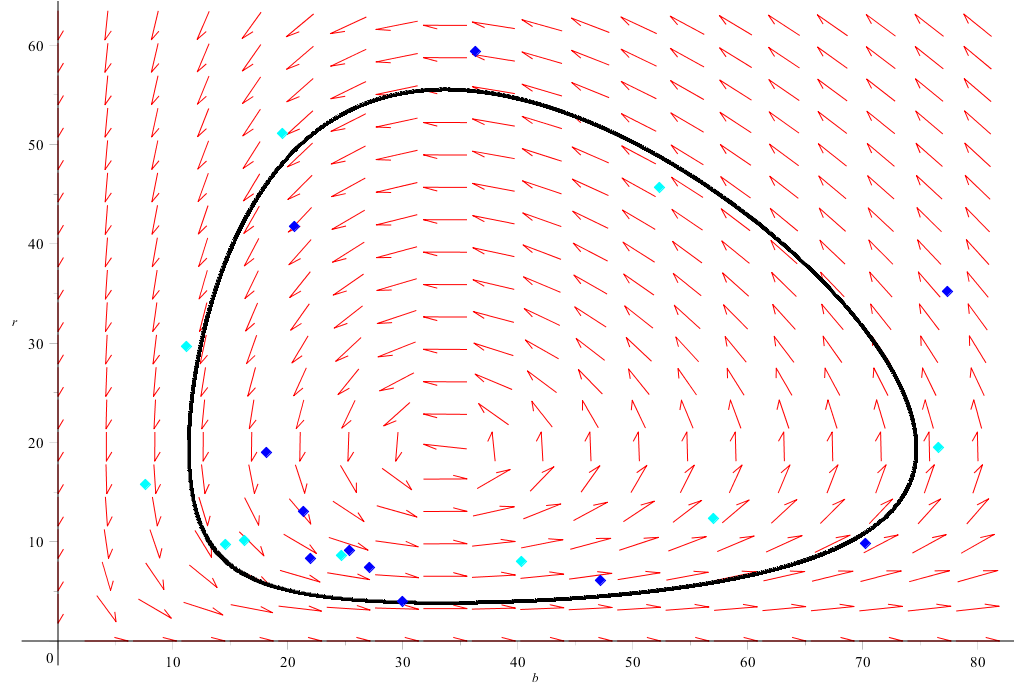
\includegraphics[scale=0.6]{Images/lynx.PNG}
    \caption{De mørkeblå punkter er første cyklus og svarer til de første 11 observationer i tabel \ref{my-label}, og de lyseblå punkter er anden cyklus og svarer til de sidste 10 observationer i tabel \ref{my-label}.}
    \label{lynxfp}
\end{figure}


%\textbf{(Følgende er ikke særligt matematisk anlagt, og minder måske mere om en afgrænsning af problemstillingen end en diskussion af antagelserne. Det kan gøres mere matematisk, hvis vi finder videnskabelige artikler, der har taget forbehold for den givne antagelse, og argumenterer ud fra deres fund.)}



\section{Diskussion af Lotka-Volterra}
Dette system er, som nævnt i Indledningen, med til at afbillede en situation under visse antagelser. Det er klart, at hvis man skulle tage højde for flere arter af rovdyr, der konkurrerede om føden af en singulær art af byttedyr, så vil der skulle tilføjes en ekstra funktion for den anden art af byttedyr, men så vil alle tre populationer være indbyrdes afhængig af hinanden, og systemet bliver mere komplekst. Så selvom systemet måske er med til at afbillede en mere virkelig situation for for eksempel losser og ræve, der begge søger at spise harer, så er det vanskeligere at modellere. En anden antagelse fra indledningen er, at rovdyrene har uendelig appetit, hvilket ikke er tilfældet i virkeligheden. Der kan dog argumenteres for, at denne antagelse fungerer i modellen, da rovdyrene ikke altid vil støde på et byttedyr, og ligeledes vil det ikke altid være det samme rovdyr, der finder føde. Antagelse 4. og 6. fra indledningen er taget for at udelukke udefrakommende påvirkning af systemet, da der ellers vil være for mange faktorer, der skal tages højde for, og det vil ikke kunne modelleres simpelt matematisk. Den næstsidste antagelse, der vil nævnes er byttedyrsarten som eneste fødekilde til rovdyrene. Denne er taget, da rovdyrene ellers vil være delvis uafhængige af byttedyrene, og systemet vil da ikke kunne modelleres som givet i \eqref{IVPlovo}. Slutteligt er der antagelsen om, at byttedyrene altid finder rigeligt føde, og denne vil blive analyseret yderligere i det følgende, hvor en begrænset mængde af føde til byttedyrene opfattes som en kapacitetsbegrænsning. Dette ses, som en realistisk udvidelse af modellen, da der i mange økosystemer ikke er ubegrænset føde til byttedyrene. Det bemærkes, at rovdyrene også vil begrænses i det følgende. Dette gøres for at dække det generelle tilfælde.